\documentclass{article}

% to avoid loading the natbib package, add option nonatbib:
% \usepackage[nonatbib]{style}

\usepackage[final]{style}

\usepackage[utf8]{inputenc} % allow utf-8 input
\usepackage[T1]{fontenc}    % use 8-bit T1 fonts
\usepackage{hyperref}       % hyperlinks
\usepackage{url}            % simple URL typesetting
\usepackage{booktabs}       % professional-quality tables
\usepackage{amsfonts}       % blackboard math symbols
\usepackage{microtype}      % microtypography
\usepackage{verbatim}
\usepackage{graphicx}
\usepackage{amsmath}
\usepackage{bm}

\title{CS131: Tracking}

% The \author macro works with any number of authors. There are two
% commands used to separate the names and addresses of multiple
% authors: \And and \AND.
%
% Using \And between authors leaves it to LaTeX to determine where to
% break the lines. Using \AND forces a line break at that point. So,
% if LaTeX puts 3 of 4 authors names on the first line, and the last
% on the second line, try using \AND instead of \And before the third
% author name.

\author{
  Khaled Jedoui, Jamie Xie, Michelle Guo, Nikhil Cheerla. \\
  Department of Computer Science\\
  Stanford University\\
  Stanford, CA 94305 \\
  \texttt{\{thekej, jaimiex, ncheerla, mguo95\}@stanford.edu} \\
  %% examples of more authors
  %% \And
  %% Coauthor \\
  %% Affiliation \\
  %% Address \\
  %% \texttt{email} \\
  %% \AND
  %% Coauthor \\
  %% Affiliation \\
  %% Address \\
  %% \texttt{email} \\
  %% \And
  %% Coauthor \\
  %% Affiliation \\
  %% Address \\
  %% \texttt{email} \\
  %% \And
  %% Coauthor \\
  %% Affiliation \\
  %% Address \\
  %% \texttt{email} \\
}

\begin{document}

\maketitle

\section{Introduction: What is tracking?}

\subsection{Definition}

Visual tracking is the process of locating a moving object (or multiple objects) over time in a sequence. 

\subsection{Objective}

The objective of tracking is to associate target objects and estimate target state over time in consecutive video frames.

\subsection{Applications}
Tracking has a variety of application, some of which are:
\begin{itemize}
\item Human-computer interaction: Eye Tracking Systems\cite{7456615}
\item Security and surveillance\cite{1406476}
\item Augmented reality\cite{1634325}
\item Traffic control: Road transportation systems\cite{4054748}
\item Medical imaging\cite{5484176}
\end{itemize}

\subsection{Challenges}

Note, that tracking can be a time consuming process due to the amount of data that in video.
Besides, tracking relies on object recognition algorithms for tracking, which might become more challenging and prone to failure for the following reasons:

\begin{itemize}
\item Variations due to geometric changes like the scale of the tracked object
\item Changes due to illumination and other photometric aspects 
\item Occlusions in the image frame 
\item Motion that is non-linear 
\item Blurry videos or videos with bad resolution might make the recognition fail 
\item Similar objects in the scene
\end{itemize}

\section{Feature Tracking}
\label{gen_inst}

\subsection{Definition}

Feature tracking is the detection of visual feature points (corners, textured areas, ...) and tracking them over a sequence of frames (images).


\subsection{Challenges of feature tracking}

\begin{itemize}
\item Figure out which features can be tracked
\item Efficiently track across frames – Some points may change appearance over time (e.g., due to rotation, moving into shadows, etc.)
\item Drift: small errors can accumulate as appearance model is updated
\item Points may appear or disappear: need to be able to add/delete tracked points
\end{itemize}

\subsection{What are good features to track?}
What kinds of image regions can we detect easily and consistently? 
We need a way that can measure “quality” of features from just a single image. Intuitively, we  want  to  avoid smooth  regions and edges.
A solution for such a problem is to use Harris Corners. Detecting Harris corners as our key points to track guarantees small error sensitivity!

Once we detect the features we want to track, we can use optical flow algorithms to solve our motion estimation problem and track our features.

\subsection{Example}

\begin{figure}[h]
  \centering
  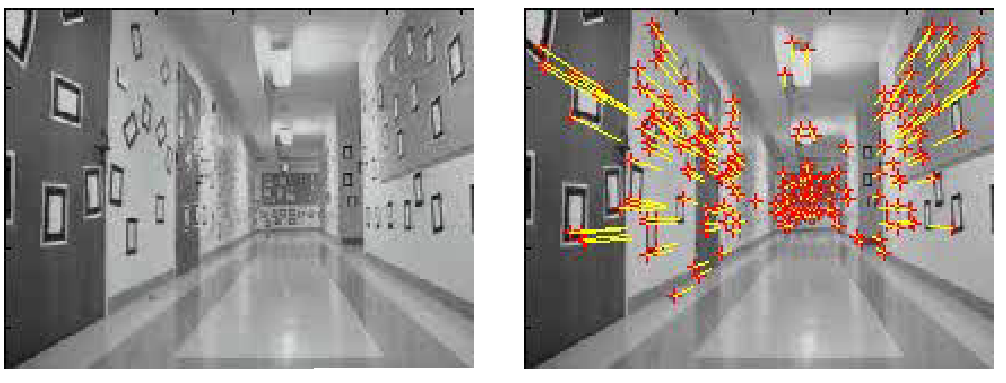
\includegraphics[width=\linewidth]{feature_track_example.PNG}
  \caption{Courtesy of Jean-Yves Bouguet–Vision Lab, California Institute of Technology}
\end{figure}

\subsection{Tracking methods}
\subsubsection{Simple Kanade–Lucas–Tomasi feature tracker}

The Kanade–Lucas–Tomasi (KLT) feature tracker is an approach to feature extraction. KLT makes use of spatial intensity information to direct the search for the position that yields the best match. Its algorithm is:

\begin{enumerate}
\item Find a good point to track (harris corner) 
\begin{itemize}
\item Harris corner points have sufficiently large eigenvalues, so the optical flow equation is solvable. 
\end{itemize}
\item For each Harris corner compute motion (translation or affine) between consecutive frames.
\item Link motion vectors in successive frames to get a track for each Harris point
\begin{itemize}
\item If the patch around the new point differs sufficiently from the old point, we discard these points.  
\end{itemize}
\item Introduce new Harris points by applying Harris detector at every (10 or 15) frames  
\item Track new and old Harris points using steps 2-3
\end{enumerate}

In the following frames from tracking videos, arrows represent the tracking motion of the harris corners. 

\begin{figure}[h]
  \centering
  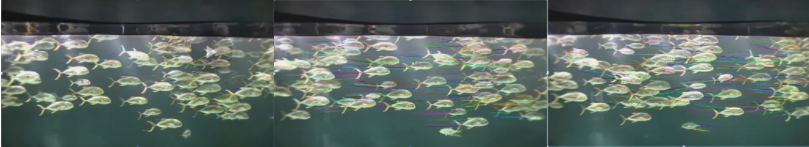
\includegraphics[width=\linewidth]{fish.png}
  \caption{Frames from fish-tracking video, courtesy of Kanade}
\end{figure}

\begin{figure}[h]
  \centering
  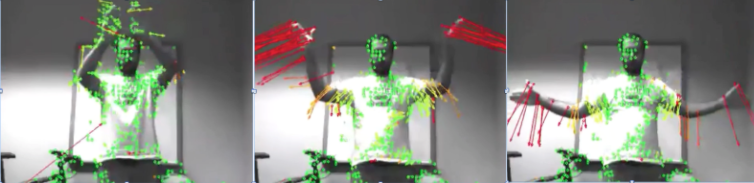
\includegraphics[width=\linewidth]{man_track.png}
  \caption{Frames from man-tracking video, courtesy of Kanade}
\end{figure}

\section{2D Transformations}
\subsection{Types of 2D Transformations}
\begin{figure}[h]
  \centering
  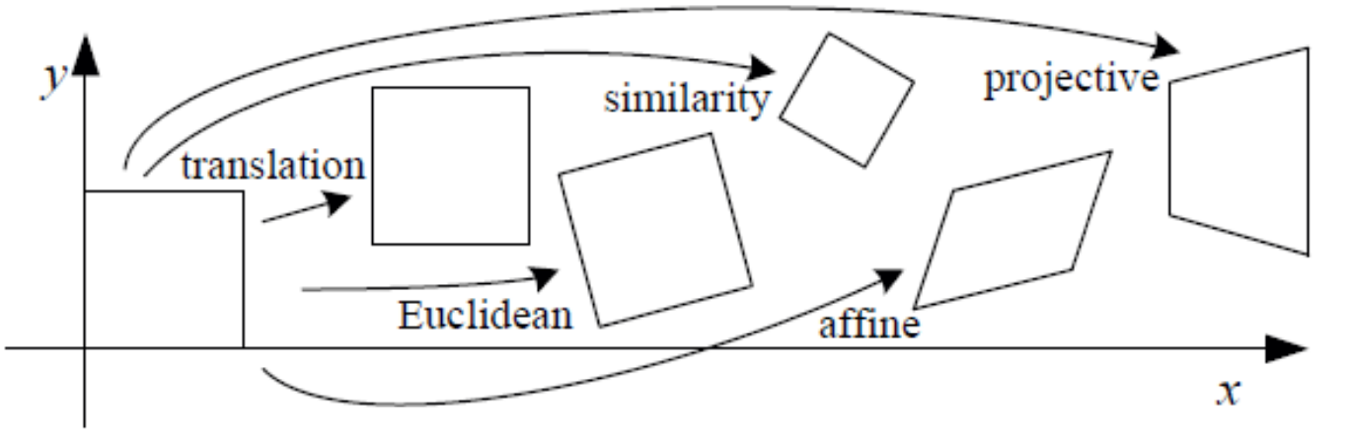
\includegraphics[width=0.8\linewidth]{trans_types.png}
  \caption{Types of 2D transformations.}
\end{figure}\label{trans_types}

There are several types of 2D transformations.
Choosing the correct 2D transformations can depend on the camera (e.g. placement, movement, and viewpoint) and objects.
A number of 2D transformations are shown in Figure \ref{trans_types}.
Examples of 2D transformations include:
\begin{itemize}
  \item \textbf{Translation Transformation}. (e.g. Fixed overhead cameras)
    \item \textbf{Similarity Transformation}. (e.g. Fixed cameras of a basketball game)
    \item \textbf{Affine Transformation}. (e.g. People in pedestrian detection)
    \item \textbf{Projective Transformation}. (e.g. Moving cameras)
\end{itemize}
In this section we will cover three common transformations: translation, similarity, and affine.

\subsection{Translation}
\begin{figure}[h]
  \centering
  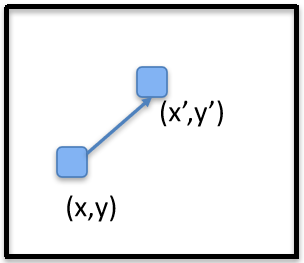
\includegraphics{translation.png}
  \caption{Translation}
\end{figure}
Translational motion is the motion by which a body shifts from one point in space to another.
Assume we have a simple point $m$ with coordinates $(x,y)$.
Applying a translation motion on $m$ shifts it from $(x,y)$ to $(x',y')$ where 
\begin{equation}
  \begin{aligned}
    x' = x + b_1 \\
    y' = y + b_2
  \end{aligned}
\end{equation}

We  can write this  as  a matrix  transformation  using homogeneous coordinates: 
\begin{equation}
  \begin{matrix}\begin{pmatrix}x' \\ y' \end{pmatrix}\end{matrix}=
  \begin{pmatrix} 1 & 0 & b_1 \\ 0 & 1 & b_2 \end{pmatrix} 
  \begin{pmatrix} x \\ y \\ 1 \end{pmatrix}
\end{equation}

Let $W$ be the above transformation defined as:
\begin{equation}
  W(\bm{x};\bm{p}) = \begin{matrix}\begin{pmatrix} 1 & 0 & b_1 \\ 0 & 1 & b_2 \end{pmatrix}\end{matrix}
\end{equation}

where the parameter vector is $p = \begin{matrix}\begin{pmatrix} b_1 \\ b_2 \end{pmatrix}\end{matrix}$.

Taking the partial derivative of $W$ with respect to $\bm{p}$ we get:
\begin{equation}
  \frac{\partial W}{\partial \bm{p}}(\bm{x}; \bm{p}) = \begin{matrix}
                        \begin{pmatrix} 1 & 0 \\ 0 & 1 \end{pmatrix}
                                       \end{matrix}
\end{equation}
This is called the Jacobian.

\subsection{Similarity Motion}
Similarity motion is a rigid motion that includes scaling and translation.

We can define the similarity as:
\begin{equation}
  \begin{aligned}
      x' &= ax + b_1 \\
      y' &= ay + b_2
    \end{aligned}
\end{equation}

The similarity transformation matrix $W$ and parameters $p$ are defined as the following:
\begin{equation}
  \begin{aligned}
    W &= \begin{matrix}
      \begin{pmatrix}
        a & 0 & b_1 \\
                0 & a & b_2
      \end{pmatrix}
    \end{matrix} \\
        \bm{p} &= \begin{matrix}
          \begin{pmatrix}
            a & b_1 & b_2
          \end{pmatrix}
        \end{matrix} ^ T
  \end{aligned}
\end{equation}
The Jacobian of the similarity transformation is then:
\begin{equation}
  \frac{\partial W}{\partial \bm{p}}(\bm{x}; \bm{p}) = \begin{matrix}
      \begin{pmatrix}
          x & 1 & 0 \\
          y & 0 & 1
      \end{pmatrix}
  \end{matrix}
\end{equation}
\subsection{Affine motion}
Affine motion includes scaling, rotation, and translation.
We can express this as the following:
\begin{equation}
  \begin{aligned}
    x' &= a_1 x + a_2 y + b_1 \\
        y' &= a_3 x + a_4 y + b_2
  \end{aligned}
\end{equation}

The affine transformation can be described with the following transformation matrix $W$ and parameters $p$:
\begin{equation}
  \begin{aligned}
    W &= \begin{matrix}
      \begin{pmatrix}
        a_1 & a_2 & b_1 \\
                a_3 & a_4 & b_2
      \end{pmatrix}
    \end{matrix}\\
        p &= \begin{matrix}
          \begin{pmatrix}
            a_1 & a_2 & b_1 & a_3 & a_4 & b_2
          \end{pmatrix}
        \end{matrix} ^ T
  \end{aligned}
\end{equation}

Finally, the Jacobian for affine motion is the following:
\begin{equation}
  \frac{\partial W}{\partial \bm{p}} (\bm{x} ; \bm{p}) = \begin{matrix}
    \begin{pmatrix}
      x & y & 1 & 0 & 0 & 0 \\
            0 & 0 & 0 & x & y & 1
    \end{pmatrix}
  \end{matrix}
\end{equation}

\section{Iterative KLT tracker}
\subsection{Problem formulation}

Given a video sequence, find the sequence of transforms that maps each frame to the next frame. Should be able to deal with arbitrary types of motion, including object motion and camera/perspective motion.

\subsection{Approach}

This approach differs from the simple KLT tracker by the way it links frames: instead of using optical-flow to link motion vectors and track motion, we directly solve for the relevant transforms using feature data and linear approximations. This allows us to deal with more complex (such as affine and projective) transforms and link objects more robustly.

Steps:
\begin{enumerate}

\item{First, use Harris corner detection to find the features to be tracked.}

\item{For each feature at location $x= [x, y]^T$: Choose a feature descriptor and use it to create an initial template for that feature (likely using nearby pixels): $T(x)$.}

\item{Solve for the transform $p$ that minimizes the error of the feature description around $x_2 = W(x;p)$ (your hypothesis for where the feature's new location is) in the next frame. In other words, solve the equation $$\sum_x {[T(W(x;p)) - T(x)]^2}$$}

\item{Iteratively reapply this to link frames together, storing the coordinates of the features as the transforms are continuously applied. This should give you a measure of how objects move through frames. }

\item{Just as before, every 10-15 frames introduce new Harris corners to account for occlusion and "lost" features.}

\end{enumerate}

\subsection{Math}

We can in fact analytically derive an approximation method for finding $p$ (in Step 3). Assume that you have an initial guess for $p$, $p_0$, and $p = p_0 + \Delta p$. 

Now, 

 $$E = \sum_x {[T(W(x;p)) - T(x)]^2} = \sum_x {[T(W(x;p_0 + \Delta p)) - T(x)]^2}$$
 
 But using the Taylor approximation, we see that this error term is roughly equal to :
 
 $$E \approx \sum_x {[T(W(x;p_0)) + \nabla T \frac{\partial W }{\partial p} \Delta p - T(x)]^2}$$
 
To minimize this term, we take the derivative with regard to $p_0$ and set it equal to $0$, then solve for $p_0$.

 $$\frac{\partial E}{\partial p} \approx \sum_x {[\nabla T(\frac{\partial W }{\partial p})^T][T(W(x;p_0)) + \nabla T \frac{\partial W }{\partial p} \Delta p - T(x)]} = 0$$
 
 $$ \Delta p = H^{-1} \sum_x {[\nabla T\frac{\partial W }{\partial p}^T][T(x) - T(W(x;p_0))]}$$, where $H$ is $\sum_x [\nabla T\frac{\partial W }{\partial p}]^T [\nabla T\frac{\partial W }{\partial p}]$

By iteratively setting $p_0 = p_0 + \Delta p$, we can eventually converge on an accurate, error-minimizing value of $p$, which tells us what the transform is.
 
\subsection{Link to Harris Corner Detection}

For translation motion, $$\frac{\partial W}{\partial p} (x; p) = \begin{matrix}\begin{pmatrix} 1 & 0 \\ 0 & 1 \end{pmatrix}\end{matrix}$$, so it is easy to show that $$ H = \begin{matrix}\begin{pmatrix} I_x^2 & I_xI_y \\ I_xI_y & I_y^2 \end{pmatrix}\end{matrix}$$. However, the Harris corner detector assumes that whenever $H$ has large eigenvalues (i.e it is stably invertible), then the point within the window is a corner. Thus, corners tend to be good features for computing translations, precisely because the resulting matrices produced by corners are stably invertible.






% References
\small
\bibliographystyle{plain}
\bibliography{bibliography}
\end{document}
